\documentclass[runningheads]{llncs}
\usepackage{graphicx}
\usepackage{amsmath}

\begin{document}
\title{Redis - ESLE Report}
\author{Group 08 - Thomas Ludger (1105153)}
\authorrunning{T. Ludger}
\institute{Instituto Superior Tecnico, Lisboa, Portugal}
\maketitle
\begin{abstract}
The goal of this work is to benchmark and analyze a distributed system to assess its behavior, scalability properties, and reason about techniques to remove or mitigate bottlenecks. \textbf{Git commit 3e4494589b6ee8b8623be638d2019f89350deaea}

\keywords{Redis  \and Scalability \and Benchmark \and Distributed system \and Database \and Cache.}
\end{abstract}

\section{Introduction}
\textbf{Redis}, REmote DIctionary Server, is an extensible, open-source, very high performance key-value database management system. It is part of the NoSQL movement and aims to provide the highest performance possible. Redis is very popular in the industry and is mainly used as a cache thanks to the possibility of writing data directly to RAM. It is a very versatile and complete tool with data persistence and replication options, while remaining easy to use.

\subsection{Justification}
We choose to study the \textbf{Redis system} for several reasons. First, Redis is an interesting system because it can have two roles, both based on performance: it can be a \textbf{key-value type memory cache}, the priority of which is the speed of the response time. But it can also serve as a more classic database for simple data. By using RAM as the main memory, it allows \textbf{quick access} to this data.
On the other hand, it is a \textbf{highly scalable system}, vertically and horizontally, whose scalability properties are interesting to study and align perfectly with the rise of cloud computing.
Finally, it is a system eminently present in large companies including Twitter for managing the chronology of tweets and it is a service available in the form of cloud provider services (Amazon, GCP, etc.).

\newpage
\section{System Description}
\subsection{Redis characteristics}

\subsubsection{Key-value database}
A key-value database or key-value store uses a simple key-value method to store data. These databases contain a simple string, the key that is always unique and an arbitrary large data field, the value. 
This type of NoSQL database implements a hash table to store unique keys along with the pointers to the corresponding data values. One of the advantage is that they are easy to design and implement.

\subsubsection{Abstract data structures}
Redis is a data structure server and therefore manages a large number of data types such as:
\begin{itemize}
    \item \textbf{Strings}
    \item \textbf{Lists}: sorted by insertion order
    \item \textbf{Sets}: unordered collections of unique strings that act like programming language (Java HashSets, Python sets, etc.)
    \item \textbf{Hashes}: record types modeled as collections of field-value pairs
    \item \textbf{Sorted sets}: collections of unique strings that maintain order based on the score associated with each string
    \item \textbf{Stream}: data structure that acts as an append-only log
    \item \textbf{Geospatial indexes}: useful for finding locations within a given geographic radius or bounding box
    \item \textbf{Bitmaps}: to perform bitwise operations on strings
    \item \textbf{Bitfiel}: encode multiple counters into a string value
    \item \textbf{HyperLog}: probabilistic estimates of the cardinality of large set
\end{itemize}


\subsubsection{Persistence}
Redis stores the dataset in memory, with two different persistence methods available. The first is \textbf{snapshot}, where the dataset is asynchronously transferred from memory to disk at regular intervals as a binary dump, using the Redis RDB dump file format.
The second method is \textbf{logging}: a record of each operation that modifies the dataset is appended to an append-only (AOF) file in a background process. Redis can rewrite the append file only in the background to avoid indefinite log growth. By default, Redis writes data to a filesystem at least every 2 seconds. In the event of a complete system crash to default settings, only a few seconds of data would be lost.

\subsubsection{Replication}
Redis supports \textbf{master-slave} replication. Data from any Redis server can be replicated to any number of replicas. This allows Redis to implement a single root replication tree. This replication is useful for read (but not write) scalability or data redundancy.

\subsubsection{Clustering}
Redis can \textbf{scale horizontally} through the functionality of Redis Cluster. It allows running a Redis installation where data is automatically shared across multiple Redis nodes.
This provides some degree of availability and the ability to continue operations when some nodes fail or are unable to communicate.

\subsection{System Architecture}
For our experimentation, we decided to follow the instructions of the official Redis documentation. Our choice was to deploy a containerized infrastructure with the orchestration tool Docker Swarm. We created a Swarm Cluster and a volume and network for deploy our Redis cluster. Then, we created two services: one for the Redis master and one as a slave, for replication. Each service is set to only one replica for this first stage of the project.

This architecture was running on a Debian 11 virtual machine with \textbf{4 vCPU} and \textbf{8Go of RAM}.

\subsection{Benchmarking strategy}
To carry out the benchmark experiments, we first decided to use the tool offered by Redis, \textit{redis-benchmark} to determine the throughput of each type of request. This benchmark performed \textbf{10,000 requests} with \textbf{50 concurrent clients} and a \textbf{data size of 3 bytes} for GET and SET requests.
To deepen our study, we decided to use a well-known database benchmarking tool: \textbf{Yahoo! Cloud Serving Benchmark (YCSB)} to determine the \textbf{throughput} and the \textbf{latency} for each type of request. It is natively compatible with Redis and offers workload templates. We modified our workload for these characteristics:
\begin{itemize}
    \item 50\% of READ requests,
    \item 20\% of SCAN,
    \item 15\% of UPDATE,
    \item 15\% of INSERT
    \item data size of 1KB (10 fileds, 100 bytes each)
    \item 1000 target operations over a data set of 1000
\end{itemize}

We ran this experiment several times, varying the number of threads (concurrent clients) from 1 to 100, with a step of 5.

Alongside the YCSB benchmark, we analyzed CPU and memory usage, thanks to Docker stats.

\newpage
\section{First results}
\subsection{Redis Scalability}

To analyze the results of the benchmarks, we made different plots, with the \textit{gnuplot} tool.
The results of our first experiment with the \textit{redis-benchmark} tool, shown in \textit{Figure 2}, showed us a throughput of 6,000 to 24,000 requests per second, depending on the type of request.

Our second experiment with YCSB, plotted in \textit{Figures 3 and 4}, showed us a very high and rather odd SCAN-like write latency of up to 225ms during 100 concurrent clients. The difference results between YCSB and \textit{redis-benchmark} can be explained with the data size difference (1KB cs 3KB) and the different type of requests (ex. \textit{get} for Redis-benchmark and \textit{hmset} for ycsb).

We also plotted the throughput (\textit{Figure 5}) revealed by this experiment and we used the same data to determine the parameters of the \textbf{Universal Scalability Model} (1) equation using the \textit{esle-usl-1.0-SNAPSHOT.jar} tool:

\begin{equation} \label{eq1}
\begin{split}
X(N) & = \frac{\lambda N}{1 + \delta(N-1) + \kappa N(N-1)}
\end{split}
\end{equation}

The tool gives us these parameters results:
\begin{equation}
\lambda &= 418,36 \quad \delta &= 0,4 \quad \kappa &= 0,00074
\end{equation}

Finally, the analysis of the use of the CPU and the memory (figure 6 and 7) showed us slight variations of the CPU according to the number of threads, in particular for the CPU which can go up to 79\%. Memory is not excessively stressed.

\newpage
\subsection{Stage Pipeline}
To find a potential bottleneck and deepen our understanding of the Redis system, we tried to break down the workload requests into stages using the logs and also the official documentation in order to build a typical pipeline.

We did the two diagrams Figure 8 and Figure 9 from our understanding to explain the global working of Redis for a \textit{Get} and \textit{Set} request and the replication and persistence features.

\subsection{First bottleneck identification and mitigation}
Our multiple experiments reveal a possible bottleneck at the CPU level which quickly reaches its limits during the benchmarks.

Another possible bottleneck would be the network, which according to the Redis documentation can quickly be the main bottleneck.

To counter this problem, it is recommended to use the \textbf{pipelining} feature which groups several commands into one. We will try to determine this to improve performance.

\newpage
\section{Experimental design}
\subsection{Metrics, factors and levels}

To evaluate the performance of our Redis system, we decided to study throughput (requests per second) and latency (response time) metrics.
The selected factors and their respective levels are:

\subsubsection{Redis Cluster} Redis scales horizontally with the ability to deploy a Redis Cluster. This allows for a Redis infrastructure where data is automatically shared across multiple Redis nodes.
Thus, Redis availability is improved with the ability to continue operations when some nodes fail or are unable to communicate.
The dataset is therefore split between multiple nodes and operations can continue even if one node experiences a failure or is unable to communicate with the rest of the cluster.

So, we can establish two factors regarding clustering:
\begin{itemize}
    \item \textbf{Level -1}: standalone mode (non-cluster)
    \item \textbf{Level 1}: cluster with 3 masters and 3 slaves
\end{itemize}

\subsubsection{Persistence}: It refers to writing data to durable storage, such as a solid-state drive (SSD).
\begin{itemize}
    \item \textbf{Level -1}: no persistence
    \item \textbf{Level 1}: AOF persistence, which logs every write operation received by the server. These operations can then be replayed again at server startup, reconstructing the original dataset.
\end{itemize}

\subsubsection{overcommit\_memory value}: The kernel virtual memory acounting mode, defined by the overcommit\_memory value on the host, which is on 0 by default. By changing to 1, the kernel pretends there is always enough memory, until memory actually runs out.
\begin{itemize}
    \item \textbf{Level -1}: overcommi\_memory=0
    \item \textbf{Level 1}: overcommit\_memory=1
\end{itemize}

\subsubsection{Pipelining}: Redis pipelining is a technique for improving performance by issuing multiple commands at once without waiting for the response to each individual command. \begin{itemize}
    \item \textbf{Level -1}: no pipelining
    \item \textbf{Level 1}: pipelining
\end{itemize}

\subsubsection{Type of CPU}: We saw with our first experiments that the CPU could be a bottleneck so we will do the experiments on two differents types of CPU d'une instance Google Cloud Platform.
\begin{itemize}
    \item \textbf{Level -1}: e2-standard-8, 8vCPU
    \item \textbf{Level 1}: e2-highmem-16, 16vCPU
\end{itemize}

\subsubsection{Replication}: use of master-slave architecture for read-only replication
\begin{itemize}
    \item \textbf{Level -1}: Replication to a slave Redis server
    \item \textbf{Level 1}: No replication, no slave Redis server
\end{itemize}

\subsection{Cloud Setup}
To carry out the experiments of the various factors presented before, we decided to continue our study in the Cloud, precisely on Google Cloud Platform.
We deployed two virtual machine instances:
\begin{itemize}
    \item e2-standard-8: 8vCPUS, 16GB of RAM, europe-west9-a zone, Debian 11 image
    \item e2-highmem-16: 16vCPUS, 64GB of RAM, europe-west9-a zone, Debian 11 image
\end{itemize}

In the machines, we re-configured a Docker Swarm as well as a Redis service.

\subsection{Experiment details}

We used the \textbf{Fracitonal Factorial Design} method to do only 8 experiments with our 6 factors with 2 levels design. We did one iteration for each experience. 
We organize the results of our experiences with two tables (see annexes):
\begin{itemize}
    \item \textbf{Table 1} presents the latency and throughput results of the experiences for READ and WRITE command (respectively get and set)
    \item\textbf{Table 2} presents the sign table, the experiments configurations and the impact percentages of each factor for each metric.
\end{itemize}

The benchmark was done using the included Redis tool \textit{redis-benchmark} with 1000 requests of 1KB data and only for the GET and SET type of requests. For pipelining, we use the pipelining option of this tool with 15 requests/pipeline.
Regarding the number of thred, we choose to take experiments values of 21 threads because the first stage shows us that it s approximately with 21 threads that we have the best performances.

With these experiments, we can determine that the most important contributing factor is confounding Pipelining (D) with Clustering (A) and Persistence (B). When this option is activated, it has an impact of more than 95\% on the throughput whether it is in writing or in reading and also with an impact of more than 47\% in reading and 72\% in writing on latency.
The other factors with the most impact on read latency is Clustering with 18\%. Then, the Persistence option has an impact of 13\% on read latency and 10\% on write latency. 
Another interesting impact is the overcommit setting and the type of CPU combined with Clustering and Overcommit with an impact of 6.52\% on the write latency.


\subsection{Scalability and Performance}

From our experiences and the Redis documentation, the best performance is when the settings are:
\begin{itemize}
    \item Cluster mode
    \item Persistence enabled
    \item overcommit\_memory=1
    \item Pipelining enabled
    \item Replication enabled
\end{itemize}

We were able to determine the theoretical equation in the same way as in stage 1 with the tool \textit{esle-usl} and thanks to the data of experiment 8 which had very good performances (reach up to 500000req/s in read and 330000 in write). We plotted it using \textit{GNUplot}(see the Figure 10).

The parameters of the Universal Scalability Law determined are the following:
\subsubsection{Read}:
\begin{equation}
\lambda &= 201000 \quad \delta &= 0,51 \quad \kappa &= 0,00033
\end{equation}

\subsubsection{Write}:
\begin{equation}
\lambda &= 196529,8 \quad \delta &= 0,77 \quad \kappa &= -0,0007
\end{equation}

\section{Conclusion}

The study of the Redis system allowed us to familiarize ourselves with the concept of distributed systems as well as the performance issues to ensure correct scalability. By analyzing the characteristics and performance of Redis, through multiple tests, we were able to determine the three factors related to the \textbf{Universal Scalability Law}.  We were also able to understand the pipeline stages of a redis request.

Finally, through the fractional factorial experimental design, we were to test 6 factors and their impact on the Redis performances system. We were able to determine that the pipelining contributing factor is a really efficient feature that have the most impact on the performance system. 
It allows us to analyse the Redis sacalability properties with more details and evaluate more precisely the performance coefficient, the serial portion and the crosstalk factor for Read and Write operations.

Based on the properties and behavior of the system analyzed, we can definitely spot great qualities and a robust architecture. However, there are still room to improvement, as we could show though the report.

\newpage
\section{Annexes}
\begin{figure}
\centering
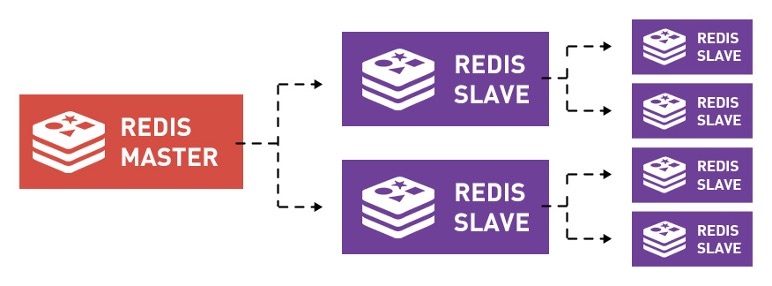
\includegraphics[scale=0.4]{images/redis-replciation.jpg}
\caption{Redis master-slave replication}
\end{figure}

\begin{figure}
\centering
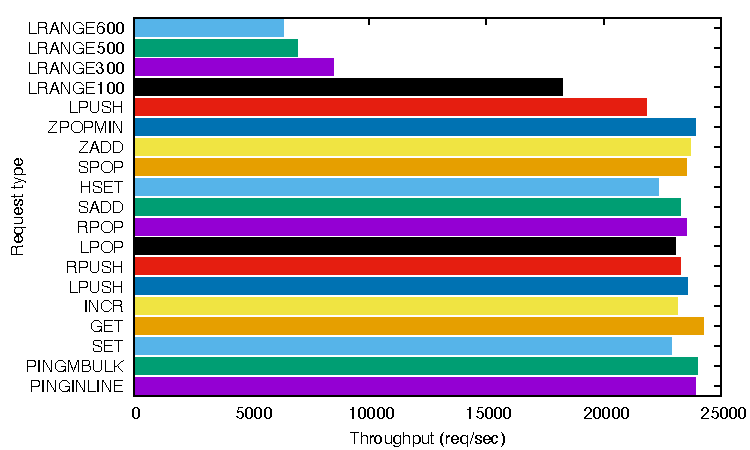
\includegraphics[scale=0.8]{images/simple_benchmark.pdf}
\caption{Throughput plot (redis-benchmark)}
\end{figure}

\begin{figure}
\centering
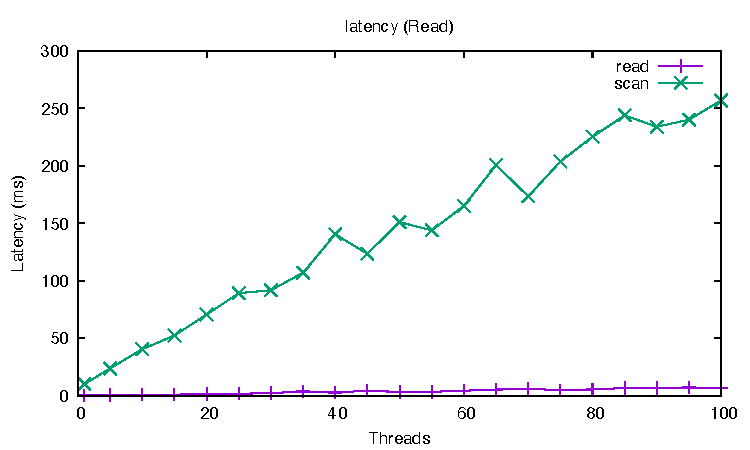
\includegraphics[scale=0.8]{images/latency 1.pdf}
\caption{Read latency plot (YCSB)}
\end{figure}

\begin{figure}
\centering
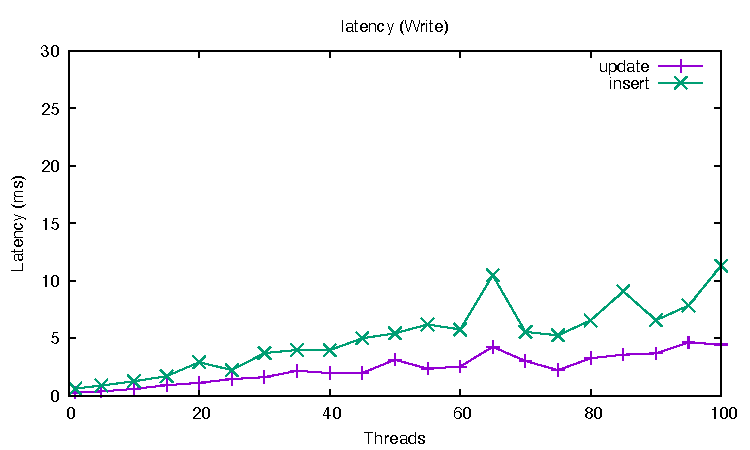
\includegraphics[scale=0.8]{images/latency 2.pdf}
\caption{Write latency plot (YCSB)}
\end{figure}

\begin{figure}
\centering
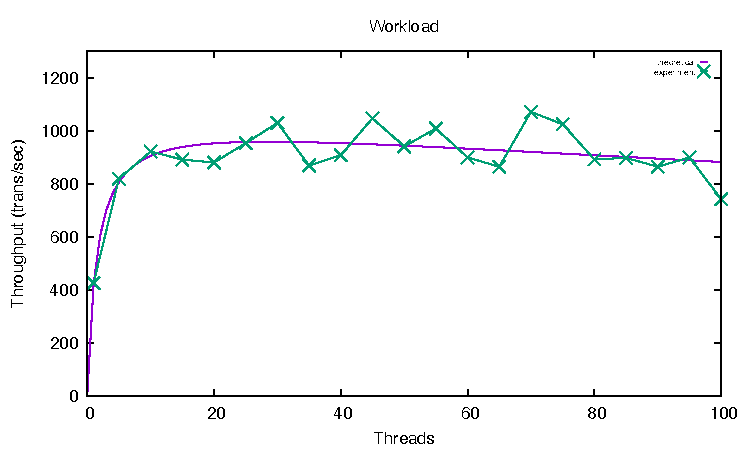
\includegraphics[scale=0.8]{images/throughput.pdf}
\caption{Throughput plot (YCSB)}
\end{figure}

\begin{figure}
\centering
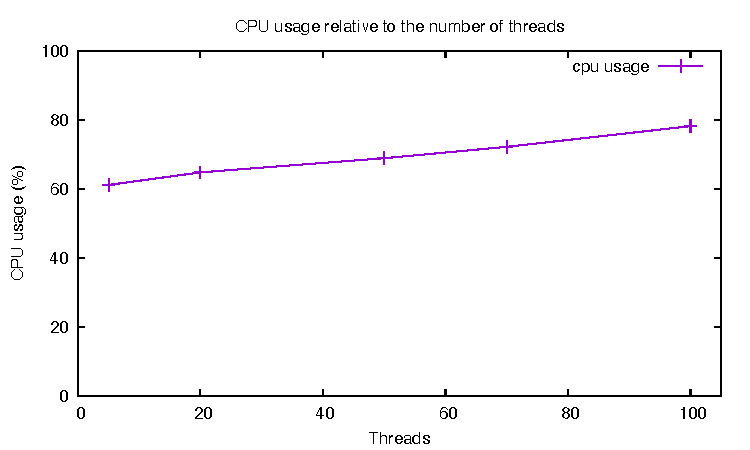
\includegraphics[scale=0.8]{images/cpu_memory_usage 1.pdf}
\caption{CPU usage during YCSB benchmark}
\end{figure}

\begin{figure}
\centering
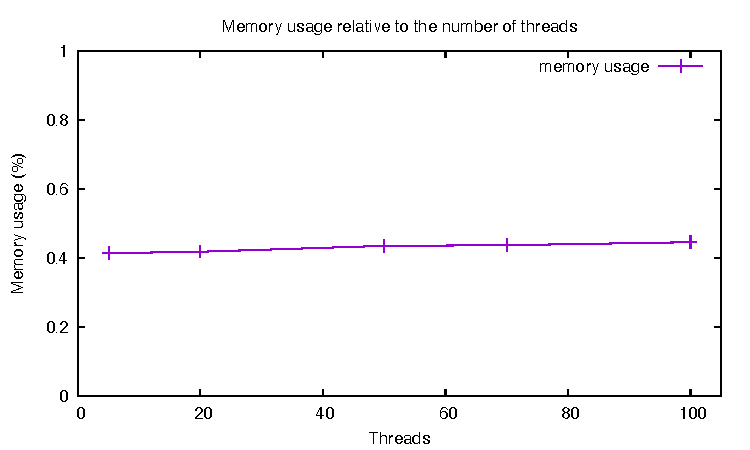
\includegraphics[scale=0.8]{images/cpu_memory_usage 2.pdf}
\caption{Memory usage during YCSB benchmark}
\end{figure}

\begin{figure}
\centering
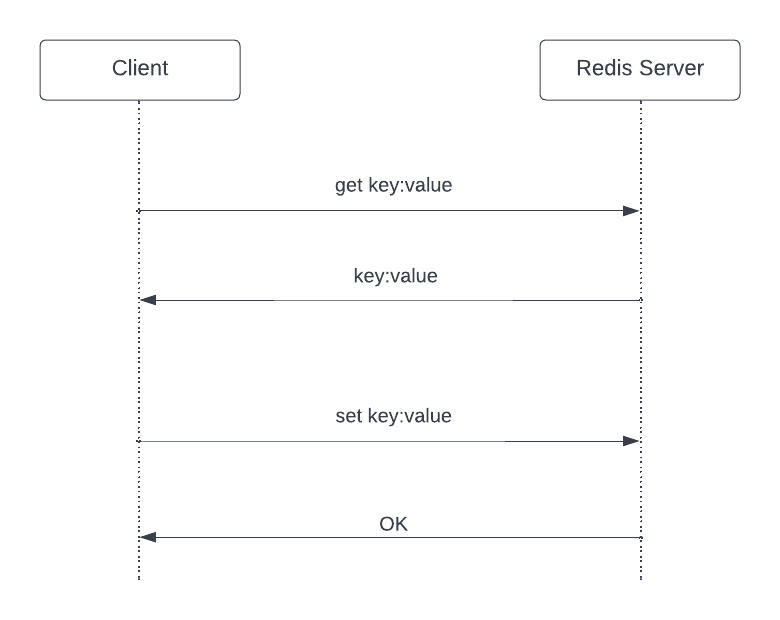
\includegraphics[scale=0.4]{images/redis1.png}
\caption{Request diagram of a Redis request}
\end{figure}

\begin{figure}
\centering
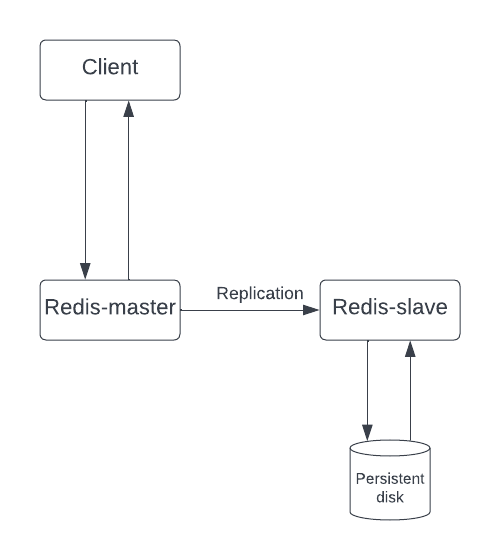
\includegraphics[scale=0.4]{images/Blank diagram-2.png}
\caption{Persistence and Replication of Redis}
\end{figure}

\newpage

\begin{table}
\caption{Experiments results (Cloud)}
\centering
\begin{tabular}{|c|l|l|} 
\hline
\multicolumn{1}{|l|}{Experience} & Mean latency (\mu s) (get-set) & Mean throughput (req/s) (get-set)  \\ 
\hline
1                                & 397 - 612                   & 502500 - 335000                    \\
2                                & 237 - 293                   & 50000 - 38461                      \\
3                                & 334 - 319                   & 35714 - 32258                      \\
4                                & 395 - 1310                  & 502499 - 251249                    \\
5                                & 469 - 811                   & 502500 - 335000                    \\
6                                & 286 - 287                   & 50000 - 55555                      \\
7                                & 430 - 384                   & 34483 - 37037                      \\
8                                & 451 - 882                   & 502499 - 335000                    \\
\hline
\end{tabular}
\end{table}

\begin{table}
\caption{Experiments results and impact of each factor for each metric}
\centering
\begin{tabular}{|l|c|c|c|c|c|c|c|} 
\hline
\multicolumn{1}{|c|}{}                                                                         & Experiment                                                         & Clustering                                                                     & Persistence                                                                    & Overcommit                                                                     & Pipelining                                                                        & CPU                                                                               & Replication                                                                        \\ 
\cline{2-8}
                                                                                               & \begin{tabular}[c]{@{}c@{}}\\1\\2\\3\\4\\5\\6\\7\\8\end{tabular}   & \begin{tabular}[c]{@{}c@{}}\textbf{A}\\-1\\1\\-1\\1\\-1\\1\\-1\\1\end{tabular} & \begin{tabular}[c]{@{}c@{}}\textbf{B}\\-1\\-1\\1\\1\\-1\\-1\\1\\1\end{tabular} & \begin{tabular}[c]{@{}c@{}}\textbf{C}\\-1\\-1\\-1\\-1\\1\\1\\1\\1\end{tabular} & \begin{tabular}[c]{@{}c@{}}\textbf{D (AB)}\\1\\-1\\-1\\1\\1\\-1\\-1\\1\end{tabular} & \begin{tabular}[c]{@{}c@{}}\textbf{E (AC)}\\1\\-1\\1\\-1\\-1\\1\\-1\\1\end{tabular} & \begin{tabular}[c]{@{}c@{}}\textbf{F (BC)}\\1\\1\\-1\\-1\\-1\\-1\\1\\1\end{tabular}  \\ 
\hline
\begin{tabular}[c]{@{}l@{}}\textbf{\textbf{READ}}\\Latency (\mu s)\\Throughput (req/s)\end{tabular} & \begin{tabular}[c]{@{}c@{}}\\2999\\2180195\end{tabular}            & \begin{tabular}[c]{@{}c@{}}\\-261\\29801\end{tabular}                          & \begin{tabular}[c]{@{}c@{}}\\221\\-29805\end{tabular}                          & \begin{tabular}[c]{@{}c@{}}\\273\\-1231\end{tabular}                           & \begin{tabular}[c]{@{}c@{}}\\425\\1839801\end{tabular}                            & \begin{tabular}[c]{@{}c@{}}\\-63\\1231\end{tabular}                               & \begin{tabular}[c]{@{}c@{}}\\31\\-1231\end{tabular}                                \\ 
\hline
\begin{tabular}[c]{@{}l@{}}\textbf{WRITE}\\Latency (\mu s)\\Throughput (req/s)\end{tabular}       & \begin{tabular}[c]{@{}c@{}}\\4898\\1419560\end{tabular}            & \begin{tabular}[c]{@{}c@{}}\\646\\-59030\end{tabular}                          & \begin{tabular}[c]{@{}c@{}}\\892\\-108472\end{tabular}                         & \begin{tabular}[c]{@{}c@{}}\\-170\\105624\end{tabular}                         & \begin{tabular}[c]{@{}c@{}}\\2332\\1092938\end{tabular}                           & \begin{tabular}[c]{@{}c@{}}\\-698\\96066\end{tabular}                             & \begin{tabular}[c]{@{}c@{}}\\-556\\71436\end{tabular}                              \\ 
\hline
\begin{tabular}[c]{@{}l@{}}\textbf{MEAN - READ}\\Latency (\mu s)\\Throughput (req/s)\end{tabular} & \begin{tabular}[c]{@{}c@{}}\\374.88\\272524.38\end{tabular}        & \begin{tabular}[c]{@{}c@{}}\\-32.63\\3725.13\end{tabular}                      & \begin{tabular}[c]{@{}c@{}}\\27.63\\-3725.63\end{tabular}                      & \begin{tabular}[c]{@{}c@{}}\\34.13\\-153.88\end{tabular}                       & \begin{tabular}[c]{@{}c@{}}\\53.13\\229975.13\end{tabular}                        & \begin{tabular}[c]{@{}c@{}}\\-7.88\\153.88\end{tabular}                           & \begin{tabular}[c]{@{}c@{}}\\3.88\\-153.88\end{tabular}                            \\ 
\hline
\begin{tabular}[c]{@{}l@{}}\textbf{MEAN - WRITE}\\Latency (\mu s)\\Throughput (req/s)\end{tabular}  & \begin{tabular}[c]{@{}c@{}}\\612.25\\177445\end{tabular}           & \begin{tabular}[c]{@{}c@{}}\\80.75\\7378.75\end{tabular}                       & \begin{tabular}[c]{@{}c@{}}\\111.5\\-13559\end{tabular}                        & \begin{tabular}[c]{@{}c@{}}\\-21.25\\13203\end{tabular}                        & \begin{tabular}[c]{@{}c@{}}\\291.5\\136617.25\end{tabular}                        & \begin{tabular}[c]{@{}c@{}}\\-87.25\\12008.25\end{tabular}                        & \begin{tabular}[c]{@{}c@{}}\\-69.5\\8929.5\end{tabular}                            \\ 
\hline
\begin{tabular}[c]{@{}l@{}}\textbf{READ}\\SS Latency (\mu s)\\SS Throughput\end{tabular}               & \begin{tabular}[c]{@{}c@{}}\\47143.5092\\423331106945\end{tabular} & \begin{tabular}[c]{@{}c@{}}\\8517.7352\\111012748.1\end{tabular}               & \begin{tabular}[c]{@{}c@{}}\\6107.3352\\111042551.2\end{tabular}               & \begin{tabular}[c]{@{}c@{}}\\9318.8552\\189432.4352\end{tabular}               & \begin{tabular}[c]{@{}c@{}}\\22582.3752\\423108483348\end{tabular}                & \begin{tabular}[c]{@{}c@{}}\\496.7552\\189432.4352\end{tabular}                   & \begin{tabular}[c]{@{}c@{}}\\120.4352\\189432.4352\end{tabular}                    \\ 
\hline
\begin{tabular}[c]{@{}l@{}}\textbf{WRITE}\\SS Latency (\mu s)\\SS Throughput\end{tabular}              & \begin{tabular}[c]{@{}c@{}}\\934553.5\\154406549421\end{tabular}   & \begin{tabular}[c]{@{}c@{}}\\52162.5\\435567612.5\end{tabular}                 & \begin{tabular}[c]{@{}c@{}}\\99458\\1470771848\end{tabular}                    & \begin{tabular}[c]{@{}c@{}}\\3612.5\\1394553672\end{tabular}                   & \begin{tabular}[c]{@{}c@{}}\\679778\\149314183981\end{tabular}                    & \begin{tabular}[c]{@{}c@{}}\\60900.5\\1153584545\end{tabular}                     & \begin{tabular}[c]{@{}c@{}}\\38642\\637887762\end{tabular}                         \\ 
\hline
\begin{tabular}[c]{@{}l@{}}\textbf{READ}\\\% Latency (\mu s)\\\% Throughput\end{tabular}               & \begin{tabular}[c]{@{}c@{}}\\100\%\\100\%\end{tabular}             & \begin{tabular}[c]{@{}c@{}}\\18.07\%\\0.025\%\end{tabular}                     & \begin{tabular}[c]{@{}c@{}}\\12.95\%\\0.025\%\end{tabular}                     & \begin{tabular}[c]{@{}c@{}}\\19.77\%\\0.00\%\end{tabular}                      & \begin{tabular}[c]{@{}c@{}}\\47.90\%\\99.95\%\end{tabular}                        & \begin{tabular}[c]{@{}c@{}}\\1.05\%\\0.00\%\end{tabular}                          & \begin{tabular}[c]{@{}c@{}}\\0.26\%\\0.00\%\end{tabular}                           \\ 
\hline
\begin{tabular}[c]{@{}l@{}}\textbf{WRITE}\\\% Latency (\mu s)\\\% Throughput\end{tabular}              & \begin{tabular}[c]{@{}c@{}}\\100\%\\100\%\end{tabular}             & \begin{tabular}[c]{@{}c@{}}\\5.58\%\\0.29\%\end{tabular}                       & \begin{tabular}[c]{@{}c@{}}\\10.64\%\\0.95\%\end{tabular}                      & \begin{tabular}[c]{@{}c@{}}\\0.39\%\\0.90\%\end{tabular}                       & \begin{tabular}[c]{@{}c@{}}\\72.74\%\\96.70\%\end{tabular}                        & \begin{tabular}[c]{@{}c@{}}\\6.52\%\\0.75\%\end{tabular}                          & \begin{tabular}[c]{@{}c@{}}\\4.13\%\\0.41\%\end{tabular}                           \\
\hline
\end{tabular}
\end{table}


\begin{figure}
\centering
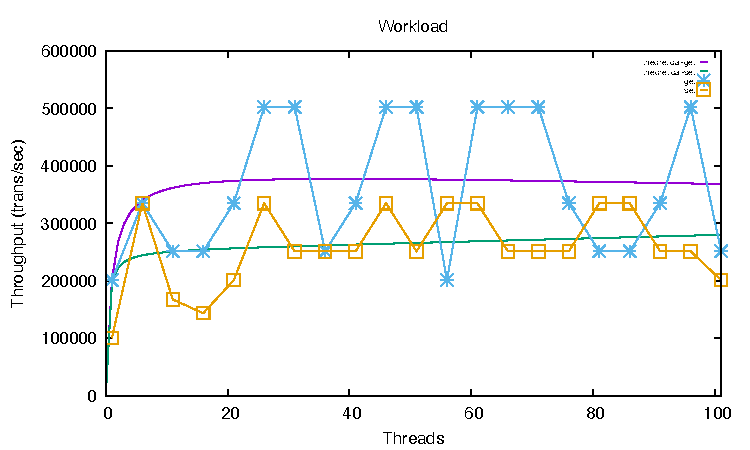
\includegraphics[scale=0.8]{images/throughput-8.pdf}
\caption{Read and Write best throughput performances}
\end{figure}

\newpage
\begin{thebibliography}{8}
\bibitem{ref_url1}
Redis Benchmark tool, \url{https://redis.io/docs/management/optimization/benchmarks/}
\bibitem{ref_url1}
Redis characteristics, \url{https://redis.io/docs/about/}
\bibitem{ref_url1}
Redis Data Types, \url{https://redis.io/docs/data-types/}
\bibitem{ref_url1}
Pipelining, \url{https://redis.io/docs/manual/pipelining/}
\bibitem{ref_url1}
Definition, \url{https://aws.amazon.com/fr/elasticache/what-is-redis/}
\end{thebibliography}

\end{document}

